\section{Privacy-preserving methods}
\label{s:types of methods}

This section clarifies methods used for privacy-preserving software.
Each subsection goes over a different step in the data life cycle, except Subsection \ref{s:DataModification}, which goes more into depth on operations that are used for the described techniques.
The life cycle is covered from capturing the data (\ref{s:DataCollectionGeneration}) until its actual use (\ref{s:DataMining}).

The following typical abstraction is used to explain the data life cycle:

\begin{itemize}

    \item 
        A \gls{DO} is an individual whose data and ultimately privacy is preferably protected 
        \cite{Aldeen2015,Jain2016,Kundeti2018}.
        Sometimes called a record owner \cite{Fung2010}.

    \item
        A \gls{DC} is an individual, a company, a government, an organization, etc. who amasses the \gls{DO}s data 
        \cite{Fung2010}.

    \item
        A \gls{DP} is comparable to \gls{DC}s, but instead of collecting data, the \gls{DP} publishes,
        for example, by sharing a data set on the web or making it accessible through an API 
        \cite{Aldeen2015,Fung2010}.

    \item
        A \gls{DR} is a third-party that executes mining on data sets published by \gls{DP}s \cite{Fung2010, Sweeney2002, Barbosa2020}.
    
\end{itemize}

Figure \ref{fig:DataCollectionDataPublishing} illustrates this abstraction: Alice, Bob, Cathy, and Doug are \gls{DO}s.
In this case, the \gls{DC} and \gls{DP} are the same.
\begin{figure}[h!]
\centering
    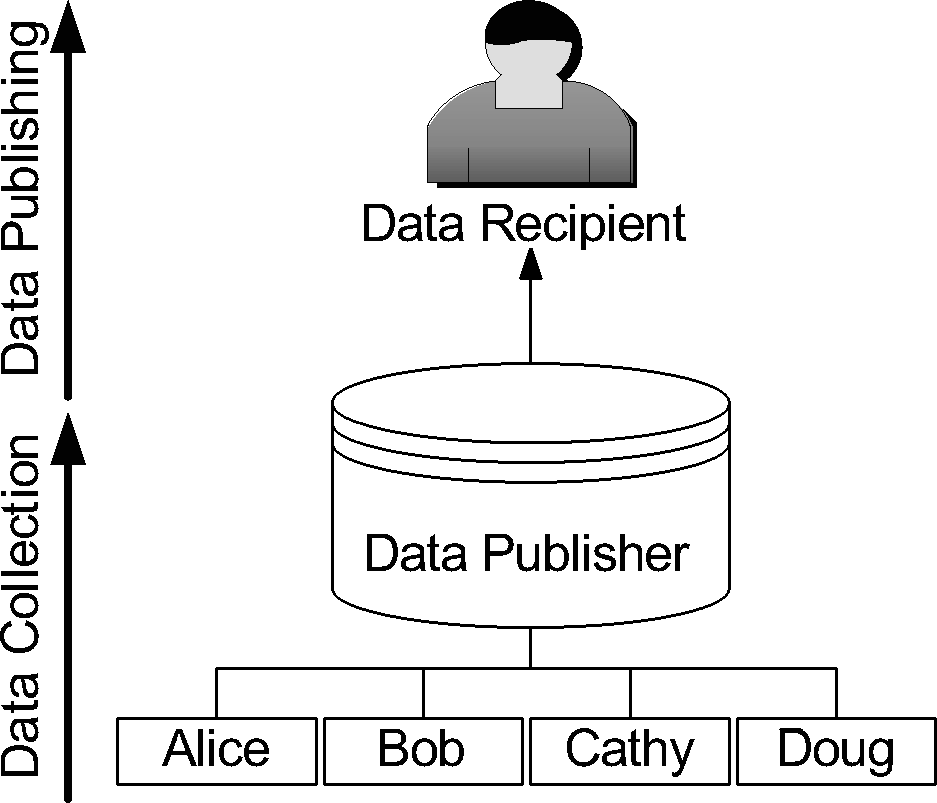
\includegraphics[width=0.5\textwidth]{figures/data-collection-and-data-publishing.png}
\caption{Data collection and data publishing \cite{Fung2010}}
\label{fig:DataCollectionDataPublishing}
\end{figure}

Furthermore, the following common terminology is used concerning the attributes of records in data sets:

\begin{itemize}

    \item
        The identifier attributes or explicit identifiers of a record contain information that can directly identify a \gls{DO}, e.g. full name and home address 
        \cite{Jain2016,Kundeti2018,Fung2010,Sweeney2002,Lu2021,Mendes2017}.

    \item 
        A \gls{QID} is a set of attributes that could lead to re-identification by combining either with or without other data from outside the data set.
        These attributes do not explicitly identify the \gls{DO} such as age and date of birth 
        \cite{Jain2016,Kundeti2018,Fung2010,Lu2021,Mendes2017}.

    \item
        Records have some attributes that contain personal information that does not explicitly identify the \gls{DO}s nor are they \gls{QID}s.
        These are called \gls{SA}, for example, sickness and religion \cite{Jain2016,Kundeti2018,Fung2010,Lu2021,Mendes2017}.

    \item
        Any other attribute containing harmless information is considered insensitive or non-sensitive \cite{Jain2016, Kundeti2018,Fung2010, Lu2021, Mendes2017}.
    
\end{itemize}


\subsection{Data collection and generation}
\label{s:DataCollectionGeneration}

% The big data life cycle exists of three parts, in the first data is collected or generated.
% Then the data is stored and lastly, the data is processed, this happens through PPDM and knowledge extraction from the data.

Data collection and generation is the first step of the data life cycle \cite{Mendes2017, Mehmood2016}.
In this phase, the data gets collected from the \gls{DO}.
This process can be active or passive. 
When the \gls{DO} knowingly gives data to the \gls{DC}, this is active data generation.
In passive data generation, the \gls{DC} gets the data from the \gls{DO} without asking for it, generally, without the \gls{DO}'s knowledge.
Several methods and techniques can provide privacy protection during the data collection phase. 
The \gls{DO} could refuse to give data to the \gls{DC} or use several tools to confirm that passively collecting the data is impossible.
This method is called access restriction \cite{Jain2016}. 

Sometimes data cannot be protected by access restrictions because the data is needed to perform specific actions. 
For example, online shopping requires users to enter their email addresses and phone numbers. 
Another method for protecting private data exists for these cases: falsifying the data.
The data is distorted such that the original information cannot be retrieved. 
To this end, \textit{Sockpuppet} can be used and tools such as \textit{MaskMe} \cite{downey_2013} are available.
This protects the online identity of the \gls{DO} by, among other things, providing a fake profile for the \gls{DO}.
This allows certain data to be used, without linkage to real users \cite{Jain2016}.  

To ensure privacy from the collector's point of view, noise or randomization \cite{Mendes2017} can be used.
Section \ref{s:NoiseRandomization} goes further into depth on noise.
% In randomization, data is distorted by adding random noise to each element of the data before sending it to the collector. 
Making sure that raw data can never be stored by the collector is an important aspect, and the usage of noise prevents this.
Otherwise, the original data could be retrieved afterwards. 

Additive noise is not significantly effective for maintaining privacy, as noise-reducing techniques are used to recover an accurate approximation of the original data. 
Noise multiplication is a more effective method since it is harder to restore the original data.
A disadvantage of both methods is their sensitivity to outliers.
More noise is needed to mask outliers, which hurts the data quality.


\subsection{Data storage}

The next step in the data life cycle is storage.
During this phase, stored data needs to be protected.
% Data storage is composed of two major parts: hardware infrastructure and data management.

Big Tech often opts for cloud computing because the amount of data they need to store is substantial.
This provides privacy benefits, such as distributed storage, but it can also come with privacy issues \cite{Mehmood2016}.
Two examples:
\begin{itemize}

    \item 
		 Even though \gls{DO}s could lose control over their data through outsourcing to the cloud,
		 this can be remedied by providing a secure computing environment and secure data storage.
    
    \item 
		 Multi-tenancy, a practice where data from different customers is located on one shared physical storage device, 
		 can make it easier for malicious users to access other users' data.
    
\end{itemize}

There are several ways to protect privacy concerning stored data.
The discussed techniques make sure that only authorized users can access their data.

\subsubsection{Identity based encryption}

The first encryption method that helps to preserve data privacy during storage is \gls{IBE} \cite{Kats2019}.
This method is similar to \gls{PKE}, but the public key depends on the identity of the user, e.g. it is based on the user's email address.
In \gls{PKE}, the user can encrypt text with a public key, resulting in what is known as a ciphertext.
This ciphertext can only be decrypted with the user's private key.
In contrast, \gls{IBE} requests the user's identity using a username and password when decrypting.
A private key generator gives the correct private key to the user to decrypt the ciphertext.
One of the problems that occur is that this method can be time-consuming when managing a wide variety of identities or huge chunks of data. 
Another disadvantage is that data can only be accessed by the \gls{DO},
while it can sometimes be useful to grant access to other users without them having the private key from the \gls{DO} \cite{Mehmood2016, Kats2019}.  

\subsubsection{Attribute based encryption}

The second method that is discussed is \gls{ABE} \cite{Jain2016, Mehmood2016}.
This belongs to \gls{PKE} where the private key depends on attributes of the \gls{DO}.
\gls{ABE} is extremely similar to \gls{IBE}, but different private keys, can be used to decrypt data that has been encrypted with the same public key.
The public key is created based on a collection of attributes instead of an identity.
Users who have these attributes are able to obtain a private key from the private key generator that can decrypt the data.
The main advantage of \gls{ABE} over \gls{IBE} is that the same data can be viewed by multiple authorized people without them having to share the same private key. 
\gls{ABE}, just like \gls{IBE}, has a considerable amount of computational overhead and is consequently quite slow \cite{Jain2016, Mehmood2016}. 

\subsubsection{Homomorphic encryption}
\label{s:HomomorphicEncryption}

A third method of protecting privacy in data storage is \gls{HE} \cite{Jain2016, Mehmood2016}.
\gls{HE} allows modifications of and computations on encrypted data without decrypting it first, contrary to \gls{IBE} and \gls{ABE}.
The output of a sequence of operations on a homomorphically encrypted data set is thus the same as if this sequence of operations were done on the data set,
while it was not encrypted.
This is beneficial as unnecessarily decrypting the data can pose privacy issues.
Again, like \gls{IBE} and \gls{ABE}, \gls{HE} requires plenty of processing power \cite{Jain2016, Mehmood2016}.

\subsubsection{Storage path encryption}

Storage path encryption \cite{Jain2016, Cheng2015} is a technique that protects private data stored on the cloud.
The data is partitioned and stored on different physical storage media, and the path to all these parts is required to obtain the data. 
Data paths, rather than the data itself, are encrypted by making use of a trapdoor function to protect this data.
This function is to calculate in one direction, but additional information is needed to calculate the inverse. 
The \gls{DO} keeps track of this information, allowing them to decrypt the path to the data and retrieve it. 

A big advantage of this technique is that it can retrieve the data rapidly because the data is divided into smaller blocks that have to be collected from the cloud.
Encrypting the path is more efficient than encrypting the data itself because of the reduced size of the path. Consequently, the computational overhead is much smaller.
By providing the additional storage path information,
it is possible to share the data with other users,
who may access the data by decrypting the proper storage path afterwards \cite{Jain2016, Cheng2015}.


\subsection{Data publishing}
\label{s:DataPublishing}

Data collection is followed by data publishing.
Fung et al. \cite{Fung2010} describe \gls{PPDP} as an \say{%
    approach to information sharing, while preserving individual privacy and protecting sensitive information%
}. \\
In \gls{DP}, \gls{DO}s share their data with either an untrusted or trusted \gls{DP}.
For the untrusted case, methods and techniques are provided in Section \ref{s:DataCollectionGeneration}.
Data is collected anonymously, i.e., the identity of the \gls{DO}s is undisclosed.
In the case of a trusted \gls{DP}, care must still be taken because the trust of the \gls{DO}s in the \gls{DP} is usually not transient to any \gls{DR}.
This means that, while an individual might entrust their data to a \gls{DP}, this trust is not implicit to \gls{DR}s.
Thus, irrespective of the model, because publishing data may result in privacy leakage, techniques and methods have been proposed to prevent this.
For the remainder of this section, trusted \gls{DP}s are assumed.

There is no single way to categorize the techniques that follow.
One way \cite{Fung2010} is to present the techniques based on the attack models they counter.
The techniques are then referred to as privacy models.
Another way \cite{Lu2021} is by the type of protection offered by these \gls{PP} techniques, which are then alternatively called privacy risk measures.
Although these two differ in perspective, they are quite related.
This section lists the most important methods and then explain what types of attacks they protect against.

Before going into depth, some more clarification is presented.
This survey \cite{Lu2021} lists three common threats:
\begin{enumerate}
    \item singling out
    \item linkability
    \item inference
\end{enumerate}

as well as four types of disclosure risks:
\begin{enumerate}
    \item identity disclosure
    \item attribute disclosure
    \item inferential disclosure
    \item membership disclosure
\end{enumerate}

Section \ref{s:DataModification} about data modification explains how the anonymization approaches are realized by digging into the operations used.
Table \ref{table:DataPublishingTechniques} summarizes many \gls{PPDP} techniques.

Finally, an attacker or adversary is an individual or an organization that seeks to violate the privacy of one or multiple \gls{DO}s, called the victims \cite{Barbosa2020}.

\begin{table*}[t] 
\small
\centering
\begin{tabular}{
    c c c c c c c
    }
    \thead{Privacy model}
    & \thead{Sanitization\\methods}
    & \thead{Record\\linkage}
    & \thead{Attribute\\linkage}
    & \thead{Table\\linkage}
    & \thead{Proba-\\bilistic\\attack}
    & \thead{References}\\
    
    \hline
    
    $k$-anonymity & Generalization, Suppression
        & x &   &   &   & \cite{Fung2010},\cite{Sweeney2002},\cite{Mendes2017}\\
    \hline
    \makecell[l]{MultiRelational\\$k$-anonymity} & Generalization, Suppression
        & x &   &   &   & \cite{Fung2010}\cite{Xu2014}\\
    \hline
    $l$-diversity & Generalization, Suppression
        & x & x &   &   & \cite{Fung2010},\cite{Mendes2017},\cite{Li_2007} \\
    \hline
     $(X, Y)$-anonymity & Generalization, Suppression
        & x &   &   &   & \cite{Fung2010},\cite{Xu2014}\\  
    \hline
    $(c,l)$-diversity & Generalization, Suppression
        & x & x &   &   & \cite{Fung2010},\cite{Mendes2017}\\
    \hline
    $t$-closeness & Generalization, Suppression
        &   & x &   &   & \cite{Fung2010},\cite{Mendes2017},\cite{Hsu_2014}\\
    \hline
    $\epsilon$-differential privacy & Randomization
        &   &   & x & x & \cite{Fung2010},\cite{Mendes2017},\cite{Hsu_2014}\\
        
\end{tabular}
\caption{\gls{PPDP} techniques}
\label{table:DataPublishingTechniques}
\end{table*}
    \subsubsection{$k$-Anonymity}
	 $k$-Anonymity is a type of privacy protection that can be used during the data publishing phase of the data life cycle.
    A data set satisfies $k$-anonymity if and only if for each set of \gls{QID}s there are at least $k$ unique records \cite{Sweeney2002}.
    Groups are at least of size $k$, thus the probability of linking a victim to a record is no more than $1/k$,
	 assuming the \gls{QID} of the victim is known to the attacker and each record in the data set represents a unique individual \cite{Fung2010}.
    If this would not be the case, multiple records would correspond to one individual and the probability of linking would be higher,
	 since $k$ records represent less than $k$ individuals.
    
		 \paragraph{Record linkage attacks}
		 \label{s:RecordLinkage}

		 A linkage attack consists of an attacker being able to link a record owner to another published record, attribute or table.
		 The assumption is that the attacker has some \gls{QID} of the victim.
		 
		 A record linkage attack can arise when the published data can be narrowed down to a small subset, called a group:
		 records with matching \gls{QID}s.
		 If the attacker has extra information, the victim's record could be identified from the group \cite{Fung2010}.

		 \paragraph{Similar techniques}
		 Improvements on $k$-anonymity exist, for example $(X, Y)$-anonymity \cite{Fung2010} which abstracts the concept of $k$-anonymity.
		 Each subset $X$, not just the \gls{QID}s, is linked to at least $k$ distinct records in the data set, with $Y$ being the sensitive attribute.            

		 MultiRelational $k$-anonymity \cite{Fung2010} extends the concept to databases consisting of multiple tables.
            
    \subsubsection{$l$-Diversity}
    $l$-Diversity is an improvement on $k$-anonymity.
    Data is $l$-diverse if there are at least l “well-represented” values that exist for sensitive attributes. 
    “Well-represented” can have different meanings that illustrate different types of $l$-diversity.
    For example, one of the interpretations is that there should be at least $l$ different values in the data \cite{Mendes2017, Li_2007}. 

		 \paragraph{Attribute linkage attacks}   
		  $l$-Diversity protects against both record and attribute linkage attacks.
		  In these attacks, the attacker may infer information from a group, as defined in Section \ref{s:RecordLinkage}.

		 Thus, a group has a set of sensitive values associated with it: all the sensitive attribute values from the records contained in the group.
		 An attribute linkage attack occurs when an attacker can infer some information about the victim from this set of sensitive values.
		 Moreover, this type of attack may still be possible if not protected against, even if record linkage attacks are prevented \cite{Fung2010}.
		 
		 \paragraph{Similar techniques}
		 An improvement on $l$-diversity is $(c,l)$-diversity.
		 This technique has the same conditions on the data as $l$-diversity,
		 but also demands that the most common values do not appear too much and the least common values are still sufficiently represented \cite{Fung2010}.
        
    \subsubsection{$\epsilon$-Differential privacy}
    The next method to ensure privacy in the publishing phase is $\epsilon$-differential privacy. 
    Differential privacy is a technique that adds randomness to the data.
    The data is still accurate enough to make overall analyses, but some information may have been adjusted. 
    Hereby $\epsilon$ is the privacy parameter that regulates the trade-off between privacy and accuracy. 
    For every entry in the data, the method decides if the value is changed.
    As a consequence, there is no certainty that the values are correct and privacy is preserved \cite{Mendes2017, Hsu_2014}.

		 \paragraph{Table linkage attacks}
			 
		 $\epsilon$-Differential privacy protects against table linkage attacks.
		 These types of linkage attacks do not assume that a victim's record is present in the published data set.
		 Contrary to record and attribute linkage, this type of attack does not have the intent to infer some information.
		 Instead, an attacker tries to infer the presence or absence of a victim in a data set \cite{Fung2010}.

    \subsubsection{$t$-Closeness}
	 The last method to provide privacy in data publishing that is discussed is $t$-closeness. 
	 In $t$-closeness, the difference between the distribution of a \gls{SA} in a group
	 and the distribution of the \gls{SA} in the database must be smaller than a certain value t \cite{Li_2007, Hsu_2014}.

		 \paragraph{Probabilistic attack}
		 $t$-Closeness protects against probabilistic attacks \cite{Fung2010}. 
		 This associated family of privacy models differs from linkage, and some mathematics are needed for clarification.
		 The attacker aims to improve their probabilistic belief about a sensitive attribute of the victim by consulting the data set.
		 The attacker's belief is given by equation \ref{eqn:BayesTheorem}.
		 The models combat this by adhering to the uninformative principle.
		 It aims to reduce the difference between the prior and posterior, see equation \ref{eqn:PosteriorPriorRelation}.

    Bayes' theorem states:
    \begin{equation}
    \label{eqn:BayesTheorem}
        P(C|\mathbf{x}) = \frac{P(C) p(\mathbf{x}|C)}{p(\mathbf{x})}
    \end{equation}
    or using terminology:
    \begin{equation}
    \label{eqn:PosteriorPriorRelation}
        posterior = \frac{prior \cdot likelihood}{evidence}
    \end{equation}

    The prior is the probability distribution of a random variable before evidence is taken into account.
    An uninformative prior has minimal influence on inference, thus making the attacker's inference harder.
    This explains the principle:
    adherence to it makes it harder for the attacker to change (i.e., improve) their belief \cite{Fung2010}.

\subsection{Data mining}
\label{s:DataMining}

\gls{DM} is the process of extracting information from a data set.
Since \gls{DM} is a buzzword, hereafter follows a delineation of the extent to which the topic is handled.
From the multitude of ways \gls{DM} may be interpreted, the focus of this paper is on:
\begin{itemize}
    \item statistics that can be done on a data set
    \item the training of \gls{ML} models on a data set
\end{itemize}

The output of a \gls{ML} model, i.e., a classifier or regressor, must also be taken into consideration when privacy preservation is important.
The output of a model could be offered to the public, another organization and other \gls{DR}s.
Attackers could try to infer sensitive information from a model.
In the following sections, techniques are presented to protect against nefarious users.
This protection can be achieved at the data or application level \cite{Mendes2017}.

    \subsubsection{Data level}

        \paragraph{Association rule hiding}
        \label{s:AssociationRuleHiding}
        
        \gls{ARH} \cite{Mendes2017, Zhang2019} is a technique that protects privacy in association rule data mining. 
        The latter is a method to identify patterns and associations in data, so rules can be formed to predict implications within the data set. 
        The rules may expose private information.
		  The main idea of \gls{ARH} is that rules that expose private information are not used, only association rules that do not disclose private information are mined.
        There are multiple approaches to apply \gls{ARH}, such as heuristic-based \gls{ARH},
		  which can be divided into a perturbation-based and a blocking-based method, reconstruction-based \gls{ARH} and metaheuristic-based \gls{ARH}. 
        These approaches are not further discussed here, but L. Zhang, W. Wang, and Y. Zhang \cite{Zhang2019} discusses them in more detail.

        \paragraph{Downgrading classifier effectiveness}
        
        Classification \cite{Mendes2017, Skarkala2021} is a method that organizes data points into different groups based on their features.
		  It links data within a group, so it can assign the right group for the specific data.
        Decision trees, clustering algorithms, Bayesian networks, and association rule mining are all processes that can be used for classifying data.
        If users can discover in which group some data is classified and what the needed features are to be classified in this group,
		  private data features may be found by nefarious users. 
        The effectiveness of the classifier can be downgraded, making it less likely that data features can be retrieved by users.

    \newpage
    \subsubsection{Application level}
    
        \paragraph{Query auditing}
        
        When queries can be directly executed on the original dataset, there are some constraints so that users can only query aggregate data and not personal data.
        There may still be some situations in which certain queries or a certain combination of queries make it possible to discover private personal data. 
        Query auditing \cite{Mendes2017} is a method to avoid such situations. 
        Some queries are denied in query auditing, to protect the private data that would be returned by those queries.

        \paragraph{Query inference control}
        
        
        Query inference control \cite{Mendes2017} is also an approach to preserve privacy when queries are executed on a dataset.
        This technique tries to solve the same problem as query auditing, but instead of prohibiting (combinations of) queries,
		  the output of the query is distorted, e.g. by adding noise, so the original private data cannot be retrieved by the queries. 
      
\subsection{Data modification}
\label{s:DataModification}

Many techniques or operations exist to modify data sets, in the context of this paper their point is to preserve the privacy of \gls{DO}s.
These operations can enable de-identification, satisfying certain \gls{PP} measures discussed in Section \ref{s:DataPublishing}, while keeping a data set valuable to a \gls{DR}.
It is this that enables data modification to foster trust between \gls{DO}s and \gls{DR}s, e.g., Big Tech companies \cite{Barbosa2020}.

Through data modification:
\begin{itemize}
    \item
        The collection of data from \gls{DO}s can be done in a \gls{PP} way, as discussed in Section \ref{s:DataCollectionGeneration}.
    \item
        The publishing of sensitive data can be done in a \gls{PP} way.
        For example, a hospital acting as a \gls{DP} could share the data with a \gls{DR} for data mining purposes.
        While guaranteeing a certain level of privacy to the \gls{DO}s through the use of \gls{PP} measures discussed in Section \ref{s:DataPublishing}.
\end{itemize}

A taxonomy is given with a few examples for each category, it is largely based on a survey \cite{Lu2021}.
An enumeration of existing operations, even if non-exhaustive, is out of the scope of this paper.
Many techniques are listed in table \ref{table:DataModificationTechniques} and a few are explained.

When these techniques are used in the context of Section \ref{s:DataPublishing}, they are called sanitization methods \cite{Mendes2017} or anonymization operations \cite{Fung2010}.

\begin{table*}[t] 
\small
\centering
\begin{tabular}{c c c}
    \thead{Category}
    & \thead{Technique}
    & \thead{References}\\
    \hline
    \multirow{5}{*}{Non-perturbative} 
        & Global recoding or generalization & \cite{Fung2010},\cite{Lu2021}\\
        & Local recoding & \cite{Lu2021}\\
        & Top-and-bottom coding & \cite{Lu2021}\\
        & Suppression or blocking & \cite{Fung2010},\cite{Lu2021}\\
        & (Sub)sampling & \cite{Lu2021}\\
    \hline
    \multirow{7}{*}{Perturbative}
        & Swapping & \cite{Fung2010},\cite{Lu2021}\\
        & Re-sampling & \cite{Lu2021}\\
        & Noise & \cite{Fung2010},\cite{Lu2021}\\
        & Aggregation or merging & \cite{Fung2010},\cite{Lu2021}\\
        & Rounding & \cite{Lu2021}\\
        & PRAM & \cite{Lu2021}\\
        & Shuffling & \cite{Lu2021}\\
        & Synthetic data generation & \cite{Fung2010}\\
    \hline
    \multirow{4}{*}{De-associative}
        & Bucketization or permutation & \cite{Lu2021},\cite{Zhang2019}\\
        & Anatomization & \cite{Fung2010},\cite{Lu2021}\\ 
        & Angelization & \cite{Lu2021}\\
        & Slicing & \cite{Lu2021}\\
\end{tabular}
\caption{\gls{PP} Data Modification}
\label{table:DataModificationTechniques}
\end{table*}

    \subsubsection{Non-perturbative}

    Despite the name of this section, this category of techniques does not modify the data.
    Instead, the data set's level of detail is reduced or information is partially suppressed, thus lowering the amount of information \cite{Lu2021}.

        \paragraph{Global recoding}
        \label{s:GlobalRecoding}

        Global recoding, also called (full-domain) generalization \cite{Fung2010, Lu2021}, changes values to be less accurate.
        Numerical values can be mapped to intervals, and the same concept can be applied to categorical values as well.
        Though for categorical values, this is less straightforward: 
        a topology of all possible values for the attribute has to be constructed.
        More specifically, this topology needs to be a tree to have a notion of what it means for a value to be more or less general.
        A parent node is then more general than its child nodes, take hobbies for example:
        

        \begin{figure}[h!]
        \centering
        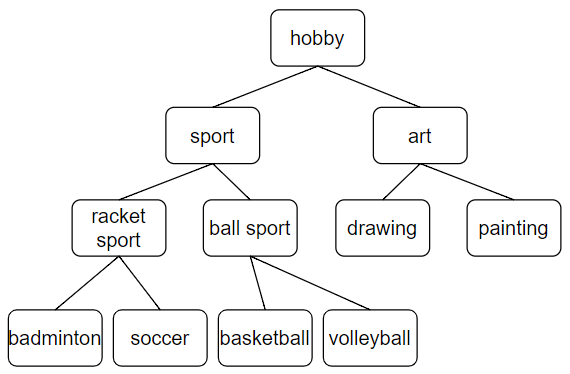
\includegraphics[width=0.5\textwidth]{figures/decision-tree.png}
        \caption{Classification of hobbies}
        \label{fig:hobbies}
        \end{figure}

        
        In essence, this technique combines values for a specific attribute into coarser categories.
        This survey \cite{Fung2010} enumerates more generalization schemes: full-domain, subtree, sibling, cell, and multidimensional.

        \paragraph{Suppression}
        \label{s:Supression}

        Suppression or blocking consists of turning attribute values into unknowns (NaNs) or special characters (`*', `?', etc.) \cite{Lu2021,Zhang2019}.
        There are multiple suppression schemes as well: tuple or record suppression, value suppression, cell or local suppression, and attribute suppression.
        Fung et al. \cite{Fung2010} and Lu et al. \cite{Lu2021} discuss these in more detail.

    \subsubsection{Perturbative}

    Perturbation-based methods are widely used heuristic techniques \cite{Mendes2017}.
    For some values of certain attributes, zeros and ones are flipped with the intent of lowering the support of sensitive rules 
	 (see Section \ref{s:AssociationRuleHiding}) in a way that the utility of the data set remains equal to a specific maximum value \cite{Mendes2017}.
    Data is distorted; in the context of \gls{DP}, this is of course done before release \cite{Lu2021}.
    
        \paragraph{Noise or randomization}
        \label{s:NoiseRandomization}

        In randomization, data is distorted by adding random noise to each element of the data set before sending it to the \gls{DC} \cite{Mendes2017}.
        Two types of noise exist: additive and multiplicative noise \cite{Lu2021, Mendes2017}.
        
        For additive noise, a noise distribution $Y$, which is most often a Normal or Gaussian distribution, is added to the data $X$. 
        The following formula applies: 
        \begin{equation}
        \label{eqn:Additive_noise}
            Z = X + Y
        \end{equation}

        Furthermore, four procedures exist for additive noise \cite{Lu2021}:
        \begin{itemize}
            \item uncorrelated noise addition,
            \item correlated noise addition,
            \item noise addition and linear transformation (e.g., Laplace noise addition) 
            \item noise addition and non-linear transformation
        \end{itemize}

        For multiplicative noise, a distribution gets multiplied with the data instead of added.
        
        \paragraph{Synthetic data generation}
        \label{s:SyntheticDataGeneration}

        New data based on statistical properties of the original data set is generated \cite{Fung2010}.

    \subsubsection{De-associative}

    The primary intent of these techniques is to disassociate the relationship between \gls{QID}s and \gls{SA}s 
    \cite{Fung2010, Lu2021}.
    The values are not changed, instead, relations are modified.
    This dissociation ameliorates the privacy of the \gls{DO}s.
    The basis for de-associative methods is groups. 
    These are records with identical \gls{QID}s.
    Each group then has particular distributions for the \gls{SA}s.

        \paragraph{Bucketization}

        Bucketization or permutation shuffles the sensitive values within each group,
		  thus keeping the distribution, yet breaking the association between \gls{QID} and \gls{SA} \cite{Fung2010}.

        \paragraph{Anatomization}

        Anatomization is a variant of bucketization that does not permute sensitive values for each group, but splits the data into two separate tables: 
        One table contains the \gls{QID}s and another the sensitive attributes.
        Both tables get a new attribute to link them: a group ID.

        The sensitive attributes' table contains the group ID, a \gls{SA}, and the number of occurrences of that \gls{SA} within the group.
        If an attacker acquires the \gls{QID} of a victim, the probability of inferring a sensitive attribute is given by the probability distribution of that specific attribute.
    
        Anatomization is not possible when a \gls{DP} wants to continuously publish more data to the data set.
        \gls{DM} discussed in Section \ref{s:DataMining} is not possible with standard techniques and more research is needed \cite{Fung2010}.

